\documentclass[11pt]{sigplanconf}
%Balanced Columns on Last Page 
\usepackage{flushend}

%Widows and Orphans 
\clubpenalty = 10000
\widowpenalty = 10000
\displaywidowpenalty = 10000

\usepackage[colorlinks,
            linkcolor=blue,
            anchorcolor=blue,
            citecolor=blue
            ]{hyperref}
\usepackage{amsmath}
\usepackage{framed}
\usepackage{breakurl}
\usepackage{multirow}
\usepackage{color}
\usepackage{listings}
\usepackage[font=small]{caption}
\usepackage{graphicx}
\usepackage{subfig}
\usepackage[boxed,ruled,nofillcomment]{algorithm2e}
%\usepackage{algorithm}
\usepackage{algpseudocode}
\graphicspath{{figure/}{figures/}{logo/}{logos/}{graph/}{graphs}}
\DeclareGraphicsExtensions{.pdf,.eps,.png,.jpg,.jpeg}


\newcommand{\tabincell}[2]{\begin{tabular}{@{}#1@{}}#2\end{tabular}}


\begin{document}


\doi{2502323.2502331} 
\conferenceinfo{CS538 2016 Spring}{University of Illinois at Urbana–Champaign}	


\newcommand{\todo}[1]{{\textbf{(TODO: #1)}}}
\newcommand{\code}[1]{{\tt#1}}
\newcommand{\reffig}[1]{Figure.~\ref{fig:#1}}
\newcommand{\refsect}[1]{Section~\ref{sect:#1}}
\newcommand{\reftable}[1]{Table~\ref{table:#1}}
\newcommand{\refalg}[1]{Algorithm~\ref{alg:#1}}
\long\def\comment#1{}



\title{Configurable and Adaptive QoS Management via SDN}

\authorinfo{Yi Zhang}
           {CS538 Advanced Computer Networks\\Department of Computer Science \\ University of Illinois at Urbana-Champaign}
			{yzhng173@illinois.edu}
\authorinfo{Qi Wang}
           {CS538 Advanced Computer Networks\\Department of Computer Science \\ University of Illinois at Urbana-Champaign}
		   {qiwang11@illinois.edu}
% make the title area
\maketitle

\begin{abstract}
In small broadband access networks (e.g., home networks), the bandwidth is usually limited. In the meanwhile,\
different applications have different Quality of Service (QoS) requirements and they all compete for the scarce bandwidth.\
Unfortunately, many users are not savvy enough to configure QoS parameters of the underlying network to meet their needs.


\end{abstract} 

\section{Introduction}
\label{sect:intro}

Communication networks nowadays have greatly improved the connectivity of the world. This connectivity
inspires and leads to a variety of online and real-time applications, like voice over IP (VoIP), video
streaming, online interactive gaming, video conferencing, etc. These applications impose diverse Quality
of Service (QoS) requirements on latency, bandwidth, jitter and error-rate. On the other hand, the
underlying networks can not provide unlimited bandwidth. According to~\cite{akamai}, the average
connection speed in the United States is 14.2Mbps. When users use multiple applications at the same time,
these applications compete for the relatively scarce bandwidth, thus leading to degradations of overall
performance.

A common approach to this problem is to prioritize applications' traffic flows so that QoS of high
priority applications can be effectively enforced. To this end, many QoS mechanisms have been proposed and
implemented (\todo{citations see flowQoS paper}). Nonetheless, these mechanisms have not been deployed in small scale broadband
access networks (e.g., home networks), for several reasons. First, many home routers have limited memory and
computation resources. Therefore, they may not be able to process and enforce complicated QoS policies
"on-the-fly"~\cite{But_Comm2018}. Second, users' demands of QoS for different applications may change in different
scenarios. For example, in a home network setting, a user may demand high definition (HD) quality of videos while
no one is playing online video games. When other users are playing online video games, she is willing to accept
standard definition (SD) quality of videos. However, many home users do not have knowledge to configure the
underlying networks to meet their needs.

Recently Software Defined Networking (SDN) has emerged as a promising approach for providing flexible network
programmability. SDN proposes to decouple the control plane from the data plane, and therefore it leaves the
existing routers and switches as simple forwarding devices. The control logic is centralized and deployed on a
server, called SDN controller, which facilitates dynamic configuration, operation and monitoring of a network.
\todo{More contents can be added here.}

In this paper, we present QoSManager, a configurable and adaptive QoS management framework based on SDN. In
QosManger, users specify high-level QoS policies (e.g., minimum bandwidth, recommended bandwidth and priority)
for different types of traffic, and QoSManager controller will dynamically assign each flow to a queue with an
appropriate sending rate to maximize the QoS utility function (\refsect{qosUF}) under the limited link capacity.
QoSManger provides an interface for modifying QoS policies at runtime (configurable) and recompute the assignments
of flows to queues when flow is added to or removed from the network (adaptive).

This paper presents several contributions. First, we design the specification language,  we take into account
that the QoS requirement for an application may change in different scenarios. Second, we design and implement
QoSManager, a configurable and adaptive QoS management framework using SDN support. Especially, we propose a novel
algorithm to assign flows to queues with appropriate rates to effectively enforce QoS. Third, we demonstrate the
effectiveness of QosManager by emulating different network scenarios.

The rest of the paper proceeds as follows. 
\refsect{related} presents related work in QoS, as well as SDN-based solutions
for home and broadband access networks. 
\refsect{qosmanager} describes the design of our system, as well as its implementation using Ryu and Open vSwitch.
\refsect{experiment} evaluates
our system in the
context of competing flows. \refsect{future} discusses future work
and concludes.

\section{Related work}
\label{sect:related}
\subsection{Traditional QoS strategies}
There are two types of strategies in traditional QoS: integrated services and differentiated services.
Integrated services are fine-grained and per-flow. 
\begin{itemize}
\item Every network element has to reserve resources for each flow.
\item Router has limited computational resources; hard to classify all app flows.
\item Not scalable.
\end{itemize}

Differentiated services~\cite{DiffServ} are more coarse-grained.
\begin{itemize}
\item Rely on the 8-bit DS field in the IP header. DiffServ routers then decide on per-hop basis how to forward packets based on their class.
\item It is static (because of the predefined number of classes) and lacks the ability to fine-tune the QoS of separate flows.
\end{itemize}


\subsection{SDN enabled QoS approach}
\subsubsection{Resource Reservation}
FlowQoS~\cite{Seddiki_HotSDN14} and EuQoS~\cite{Sharma_EWSDN14}
\subsubsection{Per-flow Routing Frameworks}
For Open-QoS~\cite{Egilmez_ASPIPA12}, after classification, high priority flows are placed on QoS guaranteed routes.

\subsubsection{Queue Management and Packet Scheduling}
\subsubsection{Policy Enforcement}

\subsection{QoS in home netowrks}
Several other approaches explore QoS in home networks.
Yiakoumis et al. proposed letting users notify the ISP about
their bandwidth needs for a given application; in this case, provisioning
occurs in the ISP’s last mile, not in the home.
Georgopoulos et al. proposed an OpenFlow-assisted framework
that improves users’ quality of experience (QoE) in
home networks for multimedia flows, subject to fairness constraints. The system allocates resources to each device
but does not perform per-application or per-flow QoS. Mortier
et al. developed Homework, a home networking platform that
provides per-flow measurement and management capabilities
for home networks. Homework allows users to monitor
and control per-device and per-protocol usage, but it does not
provide QoS support or perform any application classification.

\section{QoSManager Framework}
\label{sect:qosmanager}
In this section, we describe the design and implementation of QoSManager. We first present
an overview of the design and then describe the important components in detail.

\subsection{Overview}

\begin{figure}[htb]
\centering
\includegraphics[width=0.5\textwidth]{arch}
\caption{QoSManager architecture}
\label{fig:architecture}
\end{figure}

QosManager is implemented as an application on top of a SDN controller. As depicted in \reffig{architecture},
the main components in QosManager are: 

\begin{itemize}
  \item \emph{Web Portal}: The web portal provides an interface for users to set QoS parameters for
    different types of traffic. In addition, users could also view the real time statistical information
    about the traffic flows from the web portal.
  \item \emph{Configuration Module}: The QoS policies are stored in a QoS configuration file in YAML~\cite{yaml} format. Configuration module mainly handles the configuration file and passes the QoS policies
    to the underlying three modules (traffic classification, forwarding and control, respectively).
  \item \emph{Traffic Classification Module}: The traffic classification module classifies the application
    type for each flow. It maintains a lookup table \emph{tc\_table} where the key \emph{id} is the hash value of a
    flow's five-tuple (e.g.,source IP address, destination IP address, protocol, source port and destination port).
    The value is the application type for the flow. Each table entry is also associated with a timestamp indicating
    when the flow starts. In the current implementation, the classification is performed by querying a statically
    defined database.
  \item \emph{Forwarding Module}: The forwarding module is responsible for making forwarding decisions (e.g.,
    to which port the packet should be sent). Currently, we implement a simple L2 switch. The more sophisticated
    forwarding module is discussed in \refsect{future}.
  \item \emph{Control Module}: The control module is the core of QosManger. It dynamically computes the
    assignments of flows to queues with appropriate sending rates based on the QoS policies, the global
    information about the flows in the network.
  \item \emph{Traffic Monitor Module}: The traffic monitor module monitors the traffic flows in the network
    and constantly reports the flow status information and the port status information to the web portal.
\end{itemize}

When the first packet of a flow arrives at a switch, it does not match any entries in the flow table(s), and
it is forwarded to the controller. The Ryu SDN controller receives a \textsf{PacketIn} event and passes the
packet to QoSManager. QosManager calls the traffic classification module to classify the application type for
the flow and stores the result with a timestamp in a lookup table \emph{tc\_table}. QoSManager then invokes
the forwarding module to make the forwarding decision. The forwarding module basically implements a simple L2
switch and maintains a \emph{mac\_to\_port} table. Subsequently, QoSManager calls the control module to compute
the assignments of flows to queues with appropriate rates. Based on the forwarding decision and the assignments,
QoSManager directs the controller to send \textsf{FlowMod} messages to the switch. In addition, when a flow is
removed from a switch, the controller will receive a \textsf{FlowRemove} event and pass the flow information to
QoSManager. QosManager then invokes the control module to recompute the assignments and send \textsf{FlowMod}
messages. Note that a flow added or removed may affect the assignments of multiple flows and thus multiple
\textsf{FlowMod} messages will be sent to the switch.\todo{Add outline for subsections} 

\subsection{QoS Policy}
\label{sect:qosPolicy}

An entry in a QoS policy configuration is defined as:

\begin{lstlisting}[basicstyle=\sffamily]
<application_type>:
  minimum: <integer> Kbps
  recommended: <integer> Kbps
  priority: <integer>
\end{lstlisting}
For each type of application (e.g., video, VoIP, gaming, P2P, etc.), users needs to configure 3 parameters. The \emph{priority}
parameter specifies the users' preference for the application. The higher the value is, the more important this type of
application is. We noticed that applications such as video streaming usually have different levels of QoS. Thus, we introduce two
parameters instead of one parameter to specify the requirement for an application. The \emph{minimum} parameter specifies
the minimum bandwidth the application requires. The \emph{recommended} parameter specifies the desired bandwidth for best
performance. For example, as shown in \reftable{qos_config}, the minimum bandwidth required by VoIP is 400Kbps and the recommended
bandwidth is 1.2Mpbs. The priority of VoIP, which is 10, is higher than any other types of services, so QoSManager will first try to
satisfy the QoS requirements for VoIP services.

\subsection{Control Module}

\begin{figure}[htb]
  \centering
  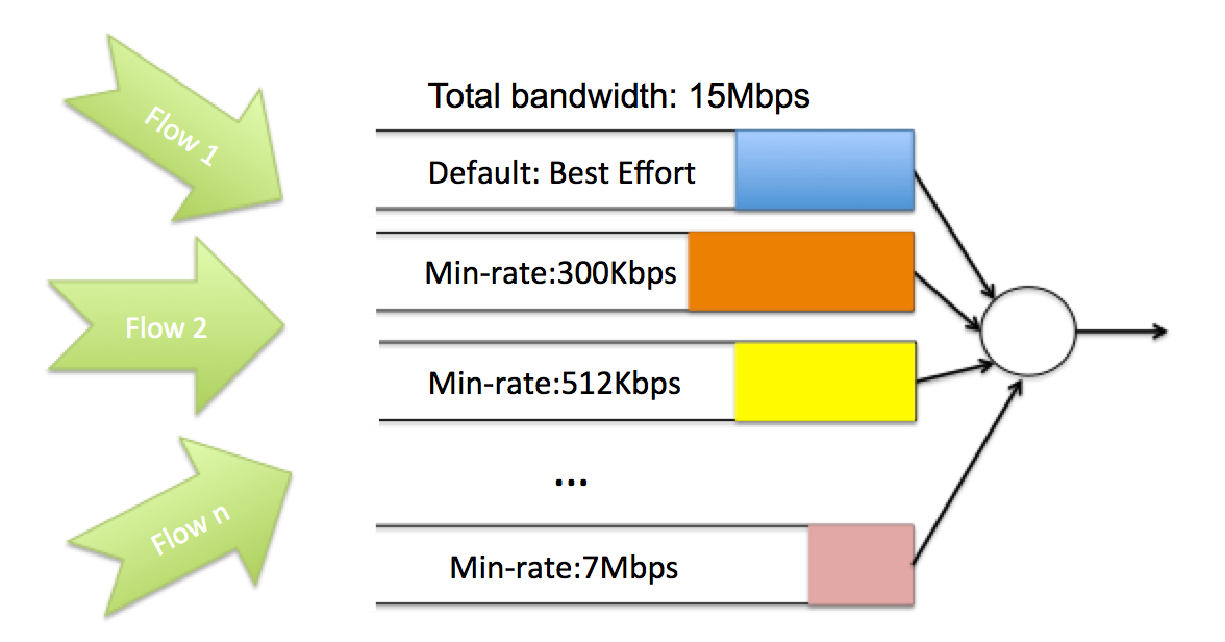
\includegraphics[width=0.5\textwidth]{assign_queue}
  \caption{QoSManager per-flow rate control.}
  \label{fig:assign_queue}
\end{figure}

The control module is the core of QoSManager. The goal of the control module is to assign an appropriate rate to each flow so that
the QoS of high priority applications can be effectively enforced. However, existing home routers do not support per-flow rate control,
and even the Open vSwitch (OVS) does not yet support per-flow QoS described in OpenFlow 1.3 specification~\cite{openflow13}. To overcome
this limitation, QosManager enables per-flow rate control by creating a list of queues with different sending rates at the ports of
the shared link \footnote{Here we assume that all the flows share a single link as shown in ~\reffig{setup}}. As shown in \reffig{assign_queue},
suppose the link capacity of the share link is \emph{C}, for each distinct bandwidth \emph{B} in the QoS policy configuration file,
we create $ N = \lfloor C / B \rfloor $ queues with minimal rate B and maximal rate C. In addition, we create a special queue $q_0$
only with maximal rate C. At runtime, QoSManager will assign each flow to a queue with an appropriate rate to control the rate of the
flow. Any flow that can not be guaranteed any level of QoS, it will be directly assigned to $q_0$.

To achieve the goal of the control module, we define the QoS utility function (\refsect{qosUF}) and propose a queue assignment
algorithm (\refsect{queueAssignAlgo}) to maximize the function under the limited link capacity.

\subsubsection{QoS Utility Function}
\label{sect:qosUF}
If the total bandwidth required by all the flows through a link exceeds the link capacity, it is obvious that the QoS requirements for
all the flows can not be fully satisfied, and we need to somehow prioritize the applications' traffic flows. In order to quantify the QoS
requirements satisfied, we assign a score to each flow. The score function for a flow \emph{f} is defined as:
\begin{equation}
\scalebox{0.9}{
  $score(f) =
    \begin{cases}
      priority       & \quad \text{if } bw(f) = \text{ recommended}\\
      0.5 \times priority & \quad \text{if } bw(f) = \text{ minimum}\\
      0              & \quad \text{otherwise}\\
    \end{cases}$
}
\end{equation}
The score function basically says that if a flow can not be guaranteed any level of QoS, it gets 0 point. To distinguish between different
levels of QoS, we give full score to a flow if it is given recommended bandwidth and partial score to a flow if it is given minimum bandwidth.
We directly use priority as score. Therefore, higher priority application flow will get higher score if it is satisfied. Based on the score
function, the goal is to maximize the QoS utility function given a shared link with the capacity \emph{C}:

\begin{equation}
\begin{split}
  U_{QoS} = \sum_{i=1}^{n} score(f_i) \\ 
  \text{under } \sum_{i=1}^{n} bandwidth(f_i) \leq C
\end{split}
\end{equation}

It is clear that high priority application flows are more likely to be assigned their recommend bandwidth \emph{all the time}, and the QoS of low
priority flows may be sacrificed. Moreover, the bandwidth allocated to high priority application will not be affected by new low priority flows
going through the link. It is possible that the total score of some lower priority flows is greater than the score of a high priority flow, and
they cost less bandwidth. In that case, the bandwidth allocated to the high priority flow will be degraded. However, users can always tune the
priority at runtime to avoid this problem.

\subsubsection{Queue Assignment Algorithm}
\label{sect:queueAssignAlgo}

The optimization of the QoS utility function is very similar to the Knapsack problem~\cite{knapsack} which can be effectively solved by dynamic
programming. However, our problem differs form the canonical bounded knapsack problem in two ways. First, in our settings, an ``object" (flow) has
two ``values" (full and partial score) and two corresponding ``volumes" (recommended and minimal bandwidth). You can only choose one of them to put
into the ``knapsack" (shared link). Second, in order to avoid fluctuation, we want to keep a flow in the same queue as long as possible. That being
said, when new objects come, and we need to reorganize the knapsack, we want to keep as many old objects in the knapsack as possible. What's more,
since the knapsack is usually much larger than the smallest object, it is not memory efficient to use the dynamic programming. Instead, we use
depth-first search (\refalg{queueAssignAlgo}) to search for the optimal assignment.

\begin{algorithm}[htp]
  \SetAlgoLined
  \SetKwFunction{algo}{algo}\SetKwFunction{proc}{dfs}
  \SetKwFunction{Sort}{Sort}
  \SetKwInOut{Input}{input}
  \SetKwInOut{Output}{output}
  \SetKwProg{myalg}{Algorithm}{}{}
  \scriptsize
  \Input{A List $flowList$}
  \Output{A Map $assign$}
  
  $flowList$ $\leftarrow$ \Sort($flowList$, key='timestamp')\;
  $flowList$ $\leftarrow$ \Sort($flowList$, key='priority', reverse)\;
  $best\_score \leftarrow 0$ \;
  $N \leftarrow flowList.length$ \;
  $dfs(0, 0, 0, newList())$ \;
  \setcounter{AlgoLine}{0}
  \SetKwProg{myproc}{Procedure}{}{}
  \myproc{\proc{index, score, bw, temp\_assign}}{

  \uIf{ $index > N$ }{
    \uIf{$score > best\_score$}{
        $best\_score \leftarrow score $\;
        $assign \leftarrow temp\_assign$ \;
    }
  }
  $f = flowList[index] $\;
  \uIf{ $bw + f.recommend < C$ }{
    $temp\_assign.append(f.id, f.recommend) $\;
    $dfs(index+1, score+f.priority, bw+f.recommend, temp\_assign)$ \;
    $temp\_assign.removeLast()$ \;
  }
  \uIf{ $bw + f.minimum < C$ }{
    $temp\_assign.append(f.id, f.minimum)$ \;
    $dfs(index+1, score+f.priority*0.5, bw+f.recommend, temp\_assign)$ \;
    $temp\_assign.removeLast()$ \;
  }
  $dfs(index+1, score, bw, temp\_assign)$ \;
  }
  \caption{Queue Assignment Algorithm}
  \label{alg:queueAssignAlgo}
\end{algorithm} 


The algorithm takes a list \emph{flowList} and the shared link capacity \emph{C} as input. The \emph{flowList} merges the tc\_table and the
QoS policy configuration. We assume that all the flows in the \emph{flowList} are successfully classified by the traffic classification module.
If a flow can not be recognized by the traffic classification module, it will be directly assigned to $q_0$. The algorithm first sort the
\emph{flowList} by timestamp and then by priority. Suppose that the sorting algorithm is stable, and we will always pick the flows in a
``first come first serve" manner if there are multiple flows of the same application type. Then the algorithm invokes depth-first search procedure
to search for the optimal assignment.

\section{Evaluation}
\label{sect:experiment}
We now present the evaluation of our system. 

\subsection{Experiment Setup}
Our experiments are done on a desktop PC with Intel(R) Core(TM) i7-2600 CPU @ 3.40GHz and 8GB RAM. The network scenario is emulated using the Mininet~\cite{mininet} framework.
It uses OS features to instantiate lightweight virtualisation of network hosts, and interconnects them with virtual switches, according to a specified topology configuration.
We implemented the control application on top of Ryu~\cite{ryu}, an open-source SDN controller.

\reffig{setup} shows our experiment setup. We configured an Internext connection to be 8 Mbps.

\begin{figure}[htb]
\centering
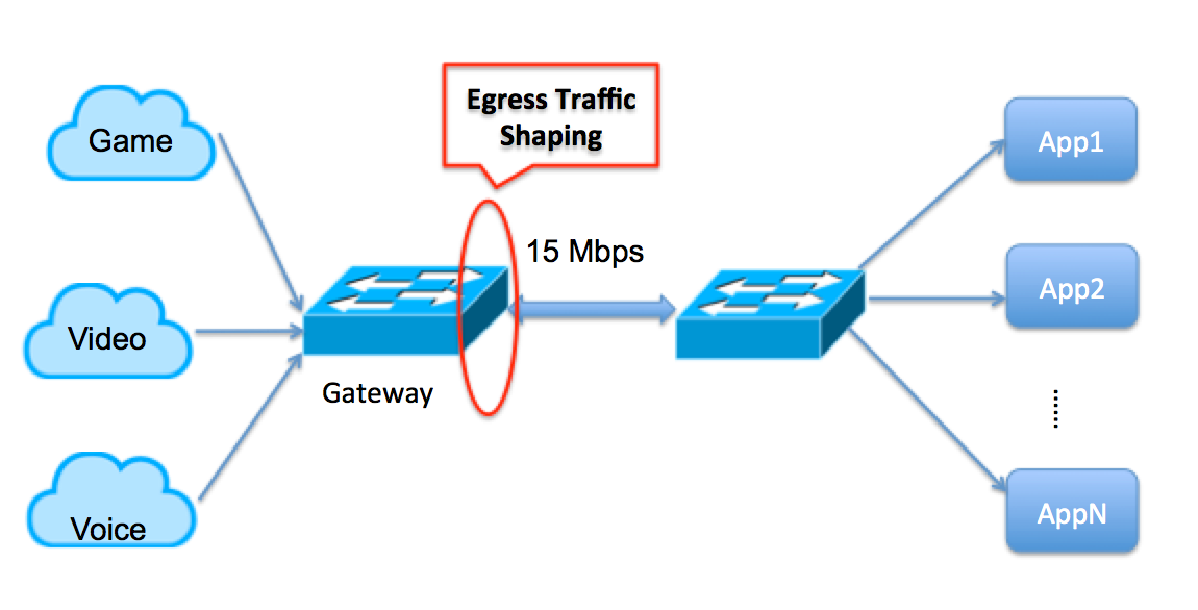
\includegraphics[width=0.5\textwidth]{exp_setup}
\caption{Experiment setup.}
\label{fig:setup}
\end{figure}

During the experiments, different hosts request different services, such as watching a video, making a VoIP call or playing a game, depending on the experiment.The QoS requirements configured for these services are shown in \reftable{qos_config}. 

\begin{table}[htb]
\scriptsize
\caption{Qos Configuration}
\begin{tabular}{|l|l|l|l|}
\hline Service type & Minimum bandwidth & Recommended bandwitdh & Priority \\
\hline
\hline VoIP & 400Kbps & 1.2Mbps & 10 \\
\hline Video & 2.5Mbps & 5Mbps & 8  \\
\hline Game & 1.5Mbps & 3Mbps & 6  \\
\hline
\end{tabular}
\label{table:qos_config}
\end{table}

We now show our system imporves the QoS of services in the face of competing traffic.
\subsubsection{Scenario 1}
In this scenario, two hosts are watching videos and one host is making a VoIP call.
The video data is sending to the hosts at rate of 5Mbps, and the VoIP data is sending to the host at rate of 1.2Mbps.
The three hosts are using the network at the same time.  

\reffig{s1_qos} illustrates the bitrates of the three services with our system, and \reffig{s1_no_qos} shows the bitrates of the three services without our system. 

\begin{figure}[htb]
\centering
\includegraphics[width=0.32\textwidth,angle=270]{s1_qos}
\caption{Bitrates of services in scenario1 with QoS.}
\label{fig:s1_qos}
\end{figure}


\begin{figure}[htb]
\centering
\includegraphics[width=0.32\textwidth,angle=270]{s1_no_qos}
\caption{Bitrates of services in scenario1 without QoS.}
\label{fig:s1_no_qos}
\end{figure}

The results show that our system provides recommended bandwidth for the VoIP flow as VoIP has higher priority than Video. 
Our system also provides recommended bandwidth for one of the video flow. While without QoS, none of three services achieve recommended bandwidth.

\begin{figure}[htb]
\centering
\includegraphics[width=0.35\textwidth,angle=270]{s1_loss}
\caption{Comparison of packets loss for VoIP with and without QoS.}
\label{fig:s1_loss}
\end{figure}

\reffig{s1_loss} shows the packet loss rate for the VoIP flow with and without QoS. As our system provides recommended bandwidth for VoIP, there is no packet loss. Without QoS, the packet loss rate is about 50 percent. Our system greatly improves the quality of VoIP call when there is competing network.

Thus, our system improves QoS of user perferred services and also reduces bitrate oscillation. 

\subsubsection{Scenario 2}
In this scenario, one host starts watching video which lasts 500s. After 50s, another host starts play a game which lasts 400s. After another 50s, another host starts another game which lasts 300s.
The video data is sending to the host at rate of 5Mbps, and the game data is sending to the hosts at rate of 3Mbps.

\begin{figure}[htb]
\centering
\includegraphics[width=0.32\textwidth,angle=270]{s2_qos}
\caption{Bitrates of services in scenario2 with QoS.}
\label{fig:s2_qos}
\end{figure}

\begin{figure}[htb]
\centering
\includegraphics[width=0.32\textwidth,angle=270]{s2_no_qos}
\caption{Bitrates of services in scenario2 without QoS.}
\label{fig:s2_no_qos}
\end{figure}

\reffig{s2_qos} illustrates the bitrates of the three services with our system, and \reffig{s2_no_qos} shows the bitrates of the three services without our system. 
With our system, as the priority of video is higher than game. The bandwidth of vidoe is not affected by the incomming game flows. Our system also provides recommended bandwidth for the first joined game flow.
Without QoS, the bandwidth of both the video and the first joined game is reduced when the second game flow comes. Also, none of the three services acheive recommended bandwidth.

Thus, in our system, services with higher priority will not be affected by services with lower priority.

\subsubsection{Scenario 3}
In this scenario, two hosts are play games. After 50s, another host starts watching a video which lasts 400s. After another 50s, another host starts making a VoIP call which lasts 300s.

\begin{figure}[htb]
\centering
\includegraphics[width=0.35\textwidth,angle=270]{s3_qos}
\caption{Bitrates of services in scenario3 with QoS.}
\label{fig:s3_qos}
\end{figure}

\begin{figure}[htb]
\centering
\includegraphics[width=0.35\textwidth,angle=270]{s3_no_qos}
\caption{Bitrates of services in scenario3 without QoS.}
\label{fig:s3_no_qos}
\end{figure}

\reffig{s3_qos} illustrates the bitrates of the four services with our system, and \reffig{s3_no_qos} shows the bitrates of the four services without our system. 
With our system, when the video flow comes in, as the priority of video is higher than game, our system reduces bandwidth of one game and provides reommended bandwidth for the video. When the VoIP flow comes in, our system again sacrifices the bandwidth of the other game to provide recommended bandwidth for VoIP as VoIP has the highest priority. When the VoIP flow ends, our system dynamically adjust bandwidth allocation, and uses the bandwidth to provide better quality for one the game.
While without QoS, when the video flow comes in, the bandwidth of both the game flows are reduced. When the VoIP flow comes in, all the bandwidth of video and games are reduced. None of the services has ever achieved recommended bandwidth.

Thus, our system will sacrifice bandwidth of service with lower priority to serve services with higher priority to satisfy the QoS requirements of user.

\section{Conclusion and Future work}
\label{sect:future}
For the future work, we plan to add more features to our system
\begin{itemize}
\item Multiple path routing
\item Time-based QoS
\item Different device QoS
\end{itemize}


%\newpage
% references section
\bibliographystyle{plain}
\bibliography{ref/ref}

\end{document}
